\chapter{Redes de neuronas}
\section{Puertas logicas}
\subsubsection{\large Elaborar las puertas lógicas anteriores mediante una red neuronal de tipo McCulloch-Pitts eligiendo convenientemente los valores de los pesos y de los umbrales} 
Puerta lógica OR:
\begin{center}
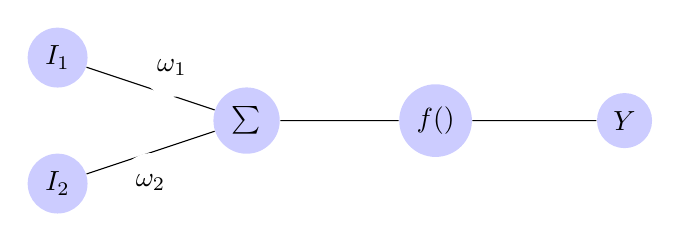
\begin{tikzpicture}[scale=.8,auto=left,every node/.style={circle,fill=blue!20}]
\node (n1) at (2,7)  {$I_1$};
\node (n2) at (2,5)  {$I_2$};
\node (n3) at (5,6)  {$\sum$};
\node (n4) at (8,6)  {$f()$};
\node (n5) at (11,6)  {$Y$};

\draw (n1) -- (n3) node [midway,fill=white]{$\omega_1$};
\draw (n2) -- (n3) node [midway,fill=white,below]{$\omega_2$};
\draw (n4) -- (n3);
\draw (n4) -- (n5);

\end{tikzpicture}
\end{center}
Parametros: $\omega_1=1$ y  $\omega_2=1$

Funcion: $$ 
y=\left \{
\begin{array}{rcl}
	1, & \mbox{si } & y \geq 1 \\
	0, & \mbox{si } & y <1
\end{array}
\right .
$$

Puerta lógica AND:
\begin{center}
	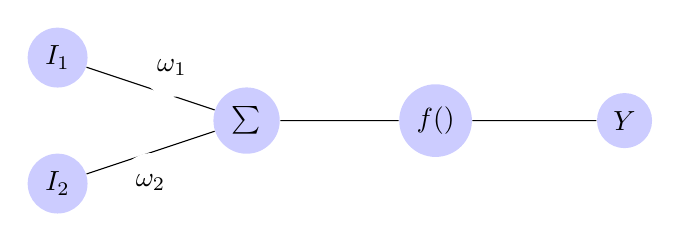
\begin{tikzpicture}[scale=.8,auto=left,every node/.style={circle,fill=blue!20}]
	\node (n1) at (2,7)  {$I_1$};
	\node (n2) at (2,5)  {$I_2$};
	\node (n3) at (5,6)  {$\sum$};
	\node (n4) at (8,6)  {$f()$};
	\node (n5) at (11,6)  {$Y$};
	
	\draw (n1) -- (n3) node [midway,fill=white]{$\omega_1$};
	\draw (n2) -- (n3) node [midway,fill=white,below]{$\omega_2$};
	\draw (n4) -- (n3);
	\draw (n4) -- (n5);
	
	\end{tikzpicture}
\end{center}
Parametros: $\omega_1=1$ y  $\omega_2=1$

Funcion: $$ 
y=\left \{
\begin{array}{rcl}
1, & \mbox{si } & y \geq 2 \\
0, & \mbox{si } & y <2
\end{array}
\right .
$$

Puerta lógica NOT:
\begin{center}
	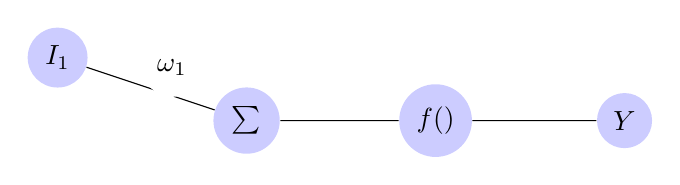
\begin{tikzpicture}[scale=.8,auto=left,every node/.style={circle,fill=blue!20}]
	\node (n1) at (2,7)  {$I_1$};
	\node (n3) at (5,6)  {$\sum$};
	\node (n4) at (8,6)  {$f()$};
	\node (n5) at (11,6)  {$Y$};
	
	\draw (n1) -- (n3) node [midway,fill=white]{$\omega_1$};
	\draw (n4) -- (n3);
	\draw (n4) -- (n5);
	
	\end{tikzpicture}
\end{center}
Parametros: $\omega_1=1$.

Funcion: $$ 
y=\left \{
\begin{array}{rcl}
0, & \mbox{si } & y \geq 1 \\
1, & \mbox{si } & y <1
\end{array}
\right .
$$

Puerta lógica XOR:
\begin{center}
	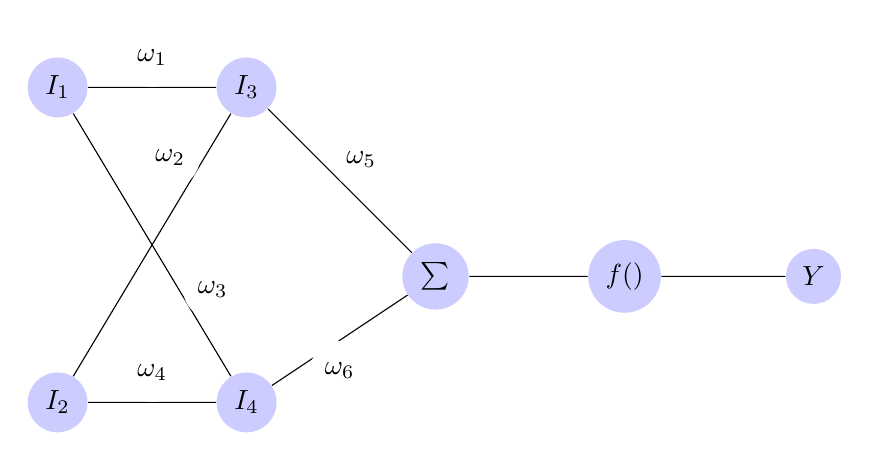
\begin{tikzpicture}[scale=.8,auto=left,every node/.style={circle,fill=blue!20}]
	\node (n6) at (-1,7)  {$I_1$};
	\node (n7) at (-1,2)  {$I_2$};
	\node (n1) at (2,7)  {$I_3$};
	\node (n2) at (2,2)  {$I_4$};
	\node (n3) at (5,4)  {$\sum$};
	\node (n4) at (8,4)  {$f()$};
	\node (n5) at (11,4)  {$Y$};
	
	\draw (n1) -- (n3) node [midway,fill=white]{$\omega_5$};
	\draw (n2) -- (n3) node [midway,fill=white,below]{$\omega_6$};
	\draw (n4) -- (n3);
	\draw (n4) -- (n5);
		\draw (n6) -- (n1)node [midway,fill=white]{$\omega_1$};
		\draw (n7) -- (n1)node [near end,fill=white]{$\omega_2$};
		\draw (n6) -- (n2)node [near end,fill=white]{$\omega_3$};
		\draw (n7) -- (n2)node [midway,fill=white]{$\omega_4$};
	\end{tikzpicture}
\end{center}
Parametros: $\omega_1=2$,$\omega_2=2$
,$\omega_3=-1$
,$\omega_4=-1$
,$\omega_6=2$
 y  $\omega_5=2$

Funcion: $$ 
y=\left \{
\begin{array}{rcl}
1, & \mbox{si } & y \geq 1 \\
0, & \mbox{si } & y <1
\end{array}
\right .
$$
\section{Hodgkin-Huxley}
\subsubsection{\large Simular el modelo de Hodgkin-Huxley y determinar el rango de I en el que aparecen oscilaciones} 
El modelo de Hodgkin y Huxley describe cómo se inician y transmiten los potenciales de acción en las neuronas. Consiste en un conjunto de ecuaciones diferenciales ordinarias no lineales que aproxima las características eléctricas de células excitables, en nuestro caso, las neuronas.


 $$I = C_m\frac{{\mathrm d} V_m}{{\mathrm d} t}  + \bar{g}_\text{K}n^4(V_m - V_K) + \bar{g}_\text{Na}m^3h(V_m - V_{Na}) + \bar{g}_l(V_m - V_l),$$

 $$\frac{dn}{dt} = \alpha_n(V_m)(1 - n) - \beta_n(V_m) n$$

 $$\frac{dm}{dt} = \alpha_m(V_m)(1 - m)  - \beta_m(V_m) m$$

 $$\frac{dh}{dt} = \alpha_h(V_m)(1 - h) - \beta_h(V_m) h$$

donde ''I'' es la corriente por unidad de area, y $\alpha_i $ and $\beta_i $ son las ratios de los canales de iones que no depende del tiempo. $\bar{g}_n$ es el valor máximo de la conductancia. '' n '', '' m '' y '' h '' son cantidades adimensionales entre 0 y 1 que están asociadas con la activación del canal de potasio, la activación del canal de sodio y la inactivación del canal de sodio, respectivamente. 

He concentrado en un grafico \ref{h} la resolucion del ejercicio, de manera que se puede observar los rangos de I que producen actividad con un grafico superpuesto. 
\begin{figure}
	\centering
	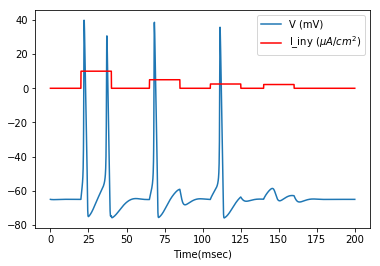
\includegraphics[width=12cm]{hodgkin}
	\caption{Representacion del modelo HH con la corriente}
	\label{h}
\end{figure}

\section{Modelo FN}

\subsubsection{\large Integrar numéricamente el modelo de FN y estudiar comportamientos dinámicos que pueden aparecer} 


El modelo de FitzHugh-Nagumo (FHN) describe un prototipo de un sistema excitable (por ejemplo, una neurona). Toma su nombre de Richard FitzHugh (1922 - 2007), quien propuso el modelo teórico en 1961, así como de J. Nagumo y otros, que construyeron un circuito electrónico equivalente.

$$
 \dot{v}=v-\frac{v^3}{3} - u + I_{\rm ext} 
 $$
 
 $$
 \tau \dot{u} = v+a-b u
 $$

Para mostrar los distintos tipos de comportamientos se han creado una serie de graficas que los exhiben: \ref{1fn}\ref{2fn}\ref{3fn}\ref{4fn}.

\begin{figure}
	\centering
	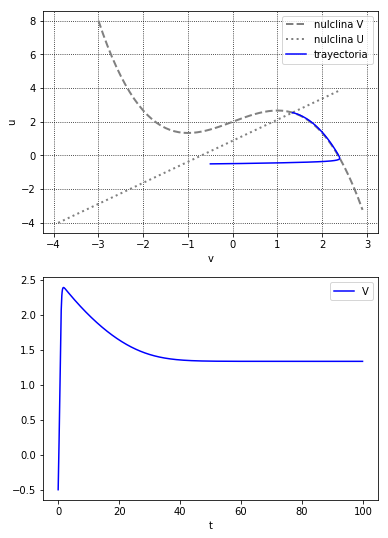
\includegraphics[width=9cm]{2}
	\caption{Tendencia al punto estable}
	\label{1fn}
\end{figure}

\begin{figure}
	\centering
	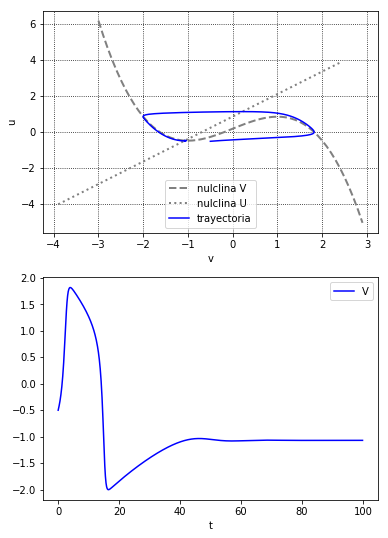
\includegraphics[width=9cm]{0-2}
	\caption{Tendencia al punto estable}
	\label{2fn}
\end{figure}

\begin{figure}
	\centering
	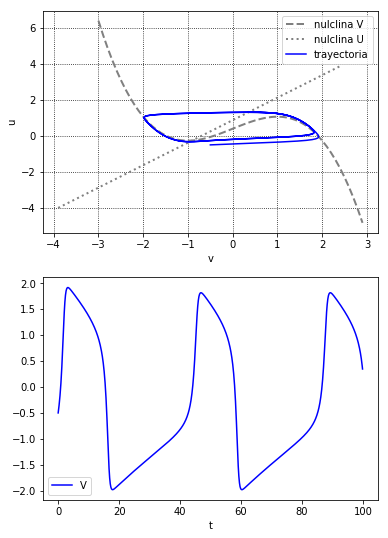
\includegraphics[width=9cm]{0-4}
	\caption{Si recibe suficiente fuerza, empiezan comportamientos periodicos}
	\label{3fn}
\end{figure}

\begin{figure}
	\centering
	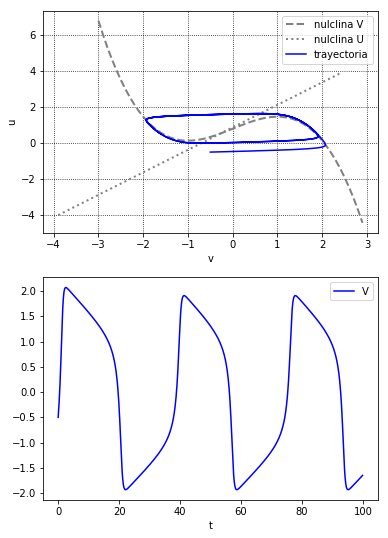
\includegraphics[width=9cm]{0-6}
	\caption{Comportamiento periodico}
	\label{4fn}
\end{figure}

\section{Modelo Tsodyks-Markram}

\subsubsection{\large Simular el modelo de Tsodyks-Markram de sinapsis dinámica y ver la forma del potencial postsináptico excitador EPSP usando por ejemplo un modelo lineal de integración y disparo para la neurona postsináptica cuando está sometida a un tren de pulsos presinápticos periódicos que llegan a una frecuencia f dada} 
Se puede consultar el script del intento en el apéndice 3, sin embargo, no ha dado resultados creíbles.










